\section{Diagramas de Estado}

De acuerdo al análisis actual, existen diferentes situaciones por las que un documento pasa a lo largo del proceso. \\

\subsection{Registro y atención de documentos entrantes}

	\begin{figure}[htbp!]
		\centering
			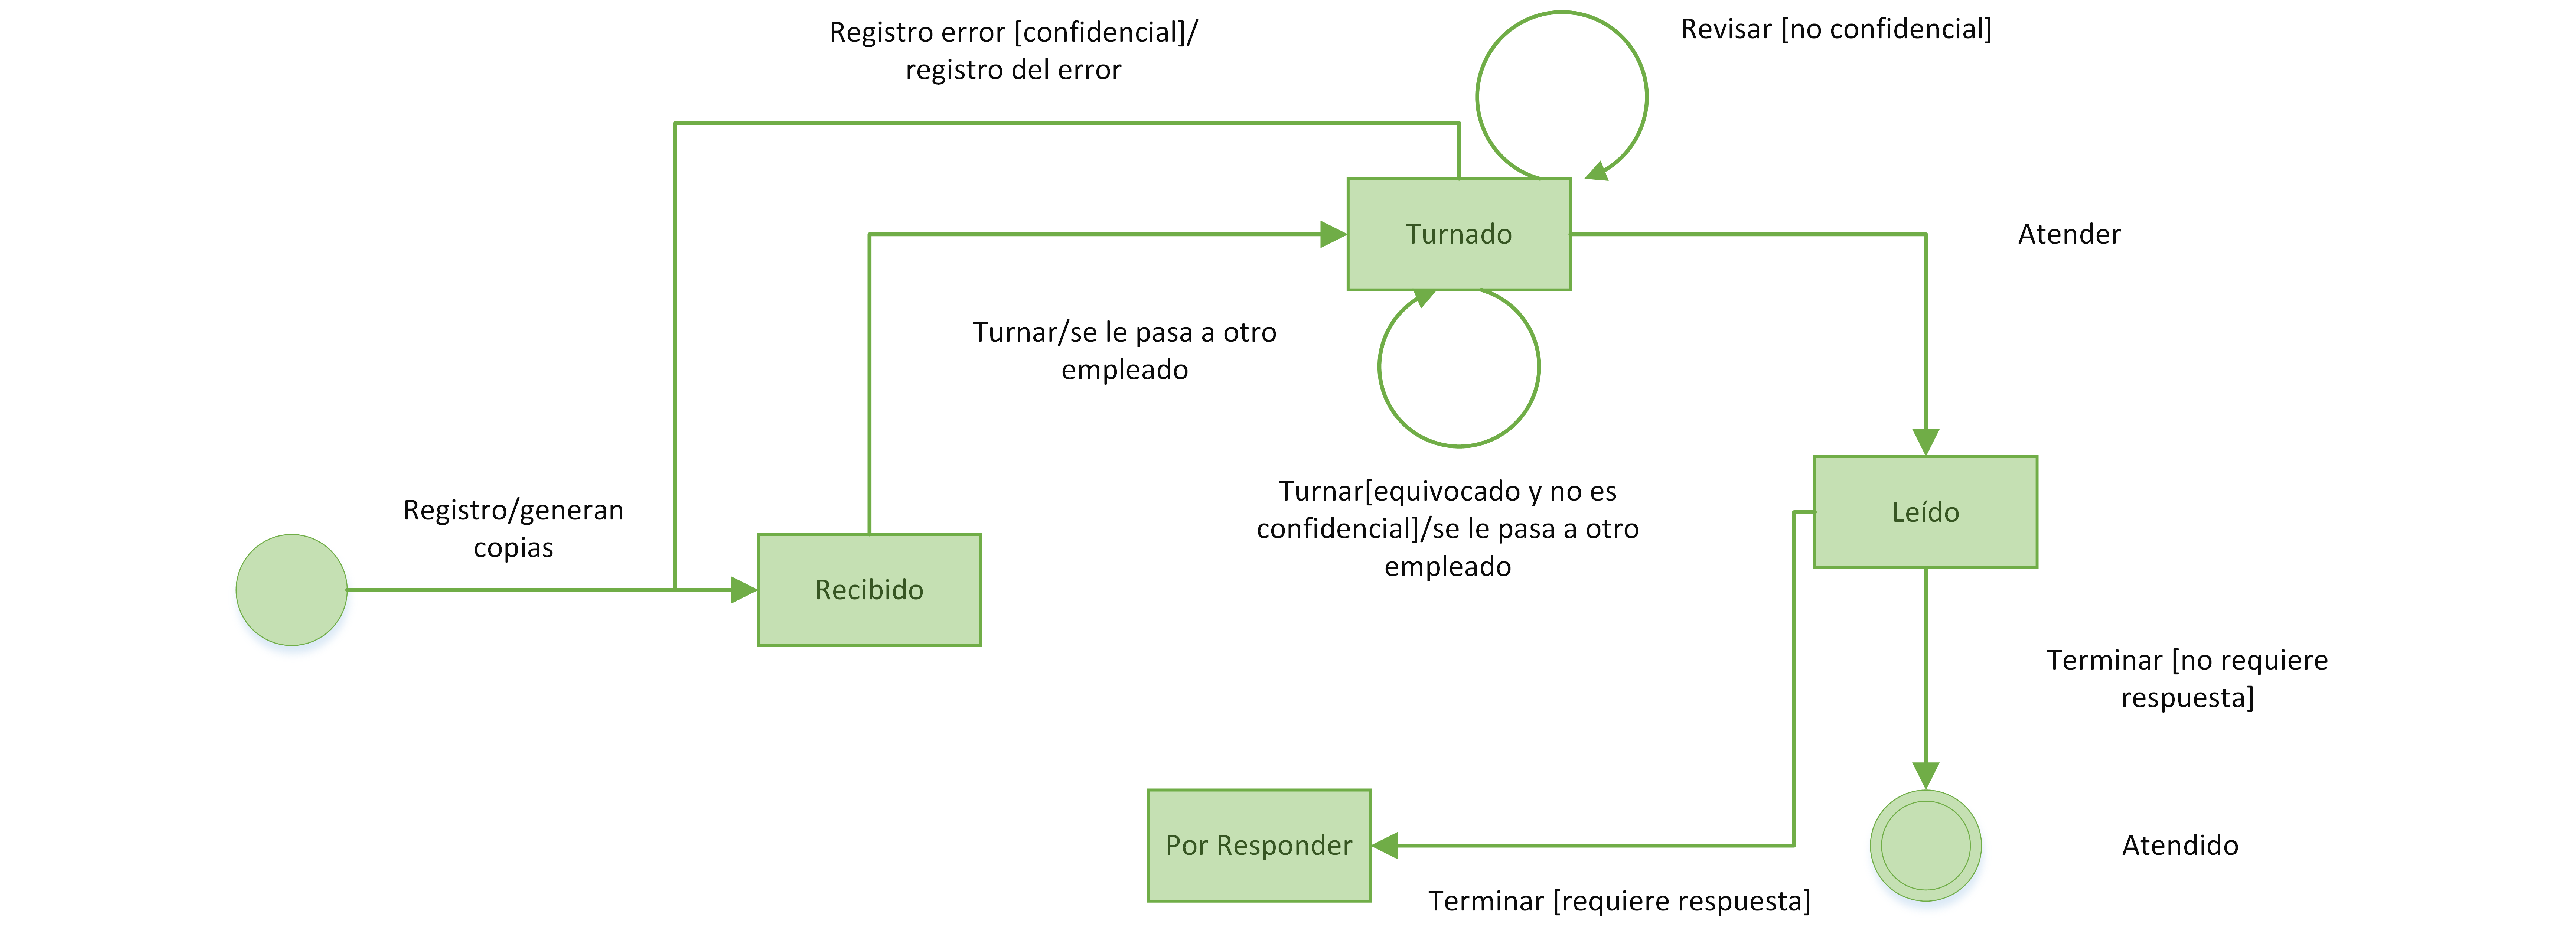
\includegraphics[width=0.8\textwidth]{images/estadosentrantes}
		\caption{Diagrama de Estados de documentos entrantes.}
	\end{figure}
	
De acuerdo con la figura 4.1 los documentos entrantes al CMPL pasan por 4 situaciones diferentes, las cuales se explican a continuación. \\ 

\textbf{Recibido}
Se denomina estado de “Recibido” cuando el oficio entrante ha sido registrado, con anexos, dentro de la aplicación. Dicho oficio sólo puede ser registrado por Oficialía de Partes y una vez finalizado el registro dicho oficio sólo puede ser visible para el Director y Oficialía de Partes.\\

\textbf{Turnado}
Se denomina estado de “Turnado” cuando un oficio entrante ha sido remitido a alguna de las áreas del CMPL o a alguna persona con atención directa. El director del centro es el que se encarga de tomar esta decisión, tomando en cuenta si el oficio se turna como documento de carácter público, confidencial o privado.\\

\textbf{Leído}
Se denomina estado de “Leído” cuando un oficio entrante de carácter informativo ha sido visto por el encargado del área o la persona a quien fue dirigido. El personal puede ver el contenido del documento viendo sus detalles dentro de la aplicación. Estos oficios son los que se registran sin que se requiera una respuesta. Este estatus sólo se considera cuando el encargado del área o la persona con atención directa han visto los detalles registrados del oficio.\\

\textbf{Por responder}
Se denomina estado de “Por responder” cuando un oficio entrante requiere una respuesta y ha sido visto por el encargado del área o la persona a quien fue dirigido. Se sabe que el oficio ha sido visto y el asunto debe ser atendido por la persona que le corresponde, pudiendo ser algún encardado de alguna de las subdirecciones, un jefe de departamento o personal en general del CMPL en caso de que sea un oficio con atención directa.\\

\textbf{Atendido}
Se denomina estado de “Atendido” cuando la respuesta de un oficio entrante ha sido enviada a la dependencia correspondiente.

\subsection{Registro de documentos salientes}
	
	\begin{figure}[htbp!]
		\centering
			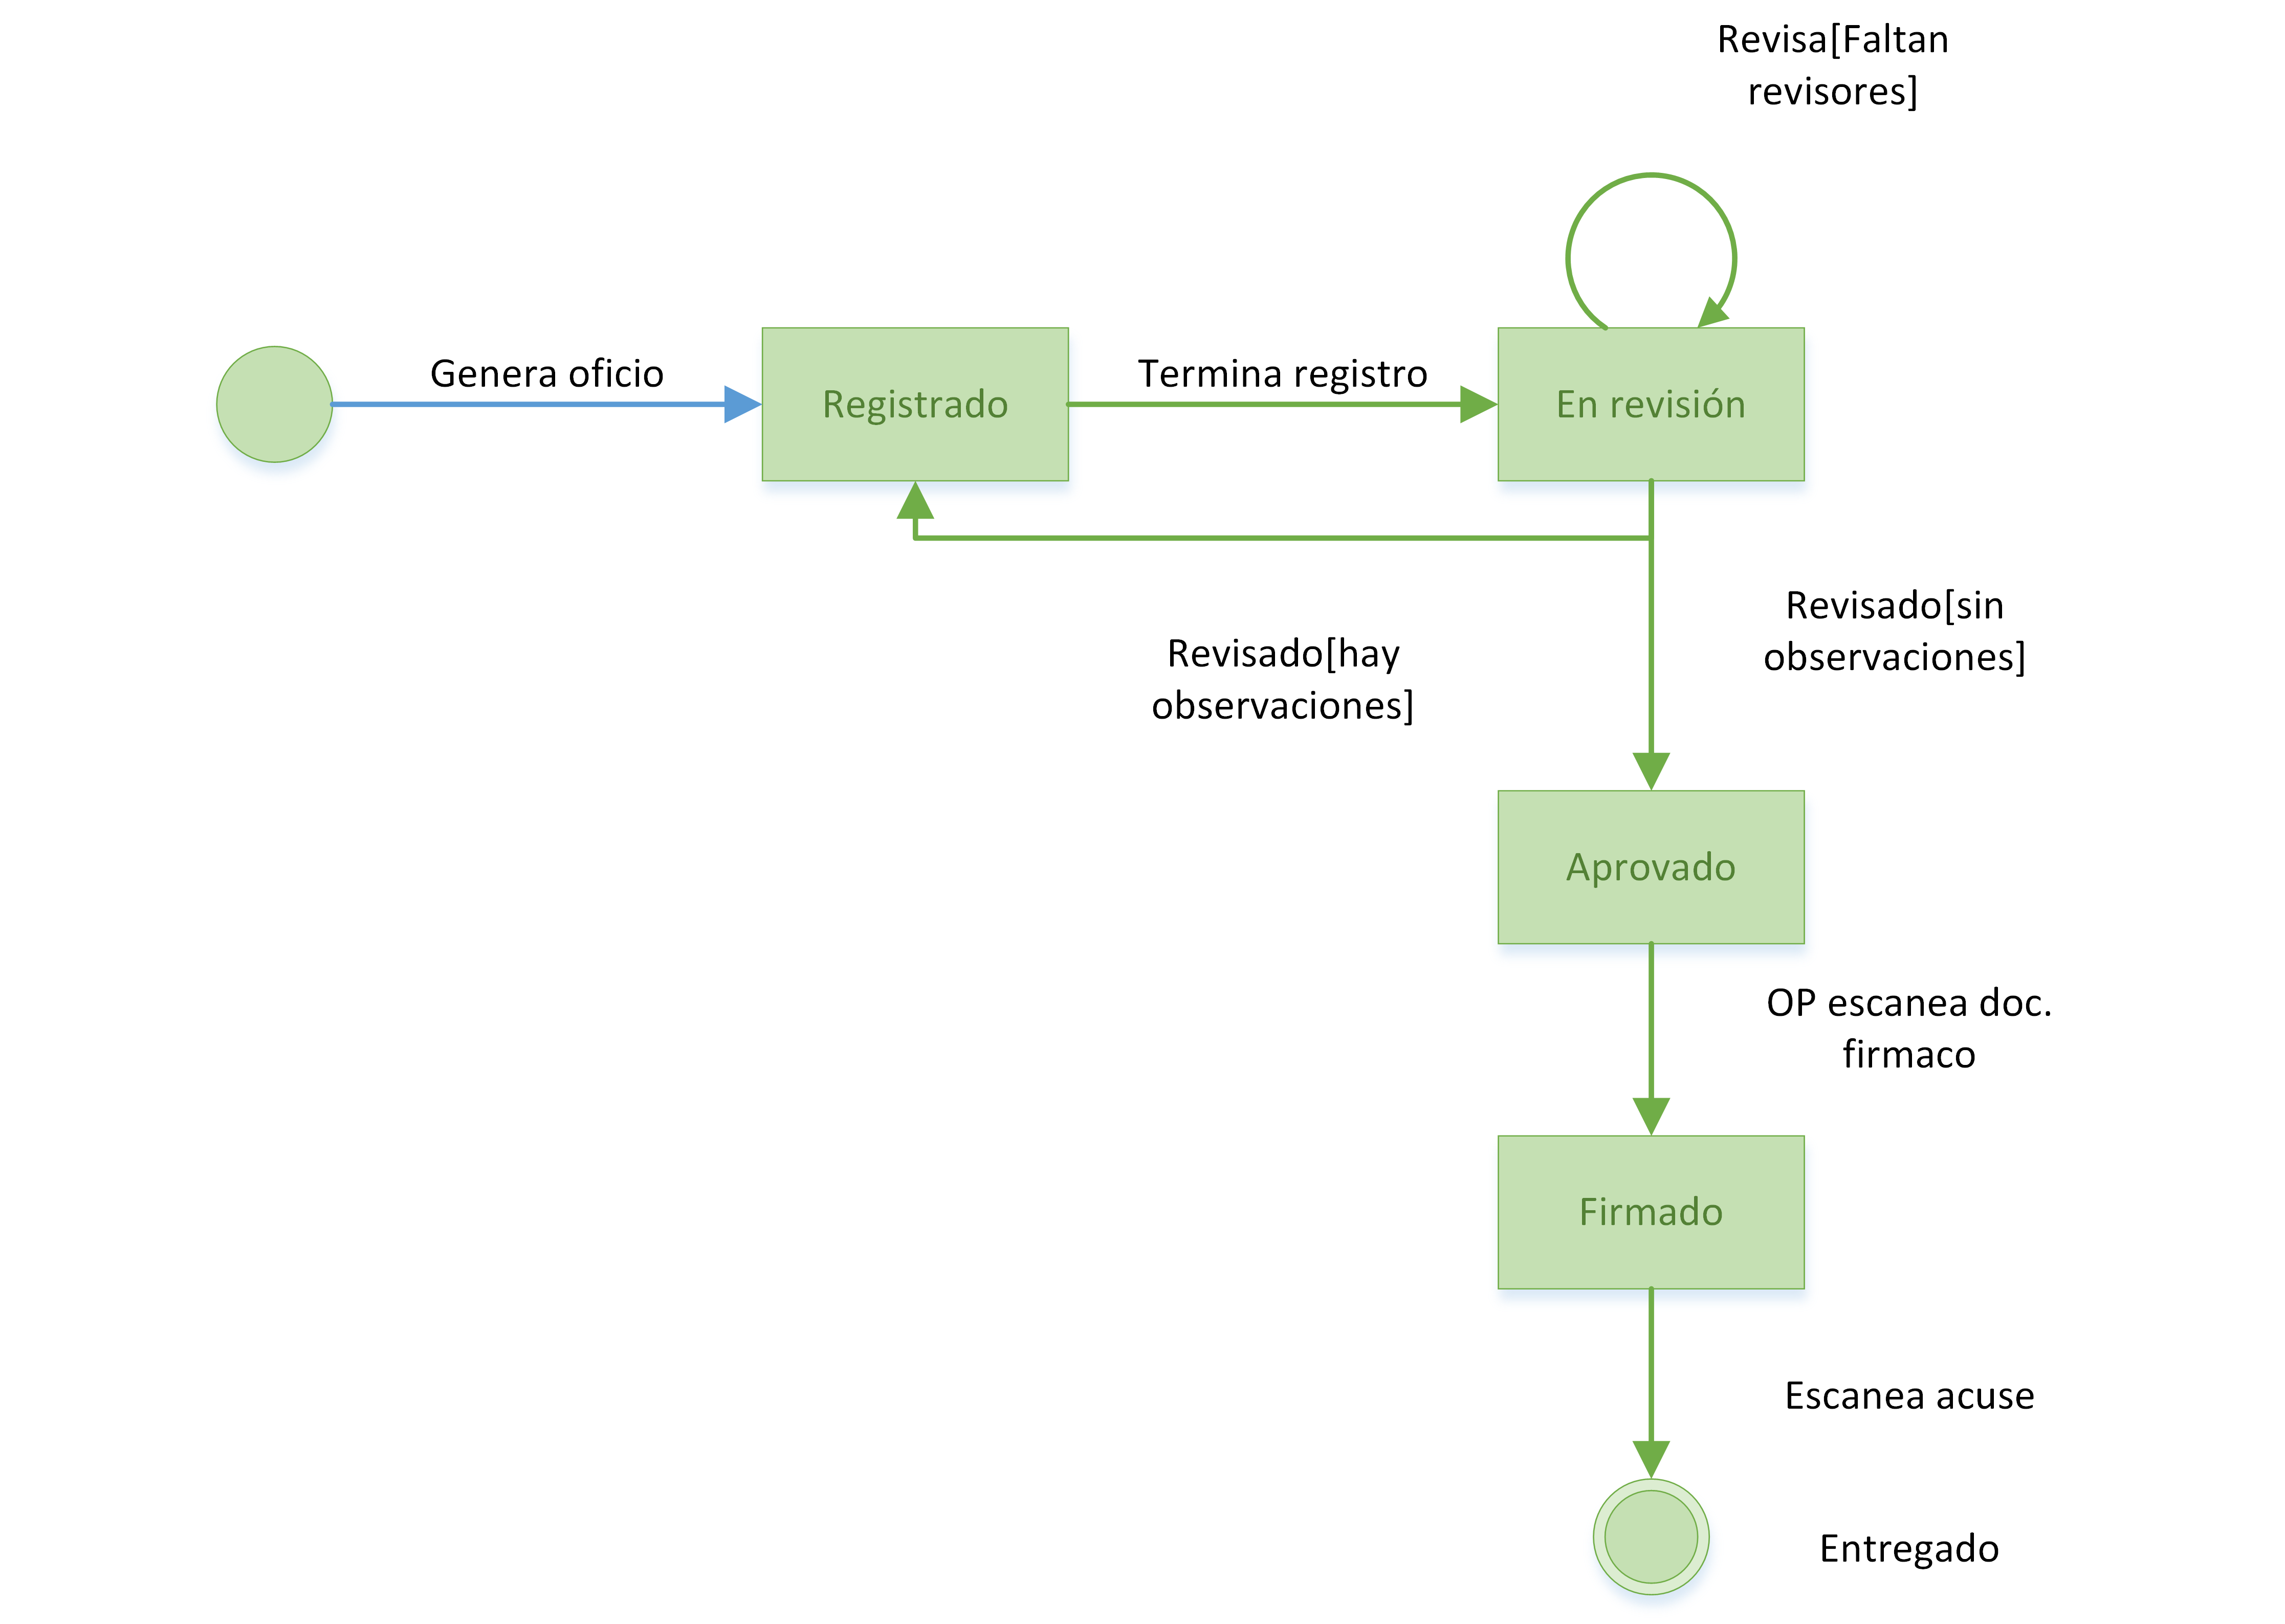
\includegraphics[width=0.8\textwidth]{images/estadossalientes}
		\caption{Diagrama de Estados de documentos salientes.}
	\end{figure}
	
De acuerdo con la figura 4.2 los documentos salientes del CMPL pasan por 4 situaciones diferentes, las cuales se explican a continuación.\\

\textbf{Registrado}
Se denomina estado de “Registrado” cuando un oficio se responde y esta registrado. Dicho oficio de respuesta es registrado por el personal que está atendiendo el asunto del oficio entrante. El personal que atiende el oficio son los encargados de las subdirecciones, los jefes de departamento y en caso de que tenga atención directa, la persona a la que se le turnó el documento.\\

\textbf{En revisión}
Se denomina estado de “En revisión” cuando un oficio ha sido registrado y su formato requiere la validación de Oficialía de Partes. Cuando un oficio se emite debe ser verificado por oficialía de partes para que cumpla con los requerimientos del formato del oficio. En este estado el oficio sólo es visible para oficialía de partes y la persona que lo redactó. En caso de que no existan observaciones al oficio por validar, podrá ser impreso para posteriormente ser firmado por el director del centro.\\

\textbf{Observaciones}
Se denomina estado de “Observaciones” cuando Oficialía de Partes ha indicado adecuaciones acerca del formato del oficio que deben ser atendidas. Hasta que no se cumpla con los requerimientos mínimos para el formato del oficio, éste no podrá ser impreso para firmar y el oficio seguirá pasando por el estado de observaciones.\\

\textbf{Firmado}
Se denomina estado de “Firmado” cuando un oficio ha sido aprobado por Oficialía de Partes y ha sido firmado por el director y está listo para ser enviado a la dependencia correspondiente.\\